\section*{Question 1: Optical Character Recognition}
\subsection*{3. Partial Training Results}

Results when using 20\% to 100\% of the training data, when validating and testing on 1000 images.

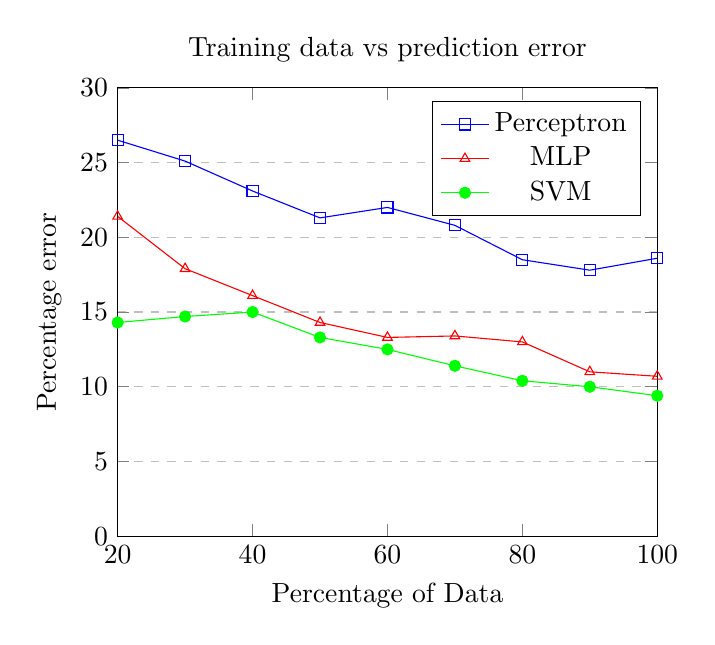
\begin{tikzpicture}
\begin{axis}[
    title={Training data vs prediction error},
    xlabel={Percentage of Data},
    ylabel={Percentage error},
    xmin=20, xmax=100,
    ymin=0, ymax=30,
    xtick={20,40,60,80,100},
    ytick={0,5,10,15,20,25,30},
    legend pos=north east,
    ymajorgrids=true,
    grid style=dashed,
]
 
\addplot[
    color=blue,
    mark=square,
    ]
    coordinates {
    (20,26.5)(30,25.1)(40,23.1)(50,21.3)(60,22)(70,20.8)(80,18.5)(90,17.8)(100,18.6)
    };
    
\addplot[
    color=red,
    mark=triangle,
    ]
    coordinates {
    (20,21.4)(30,17.9)(40,16.1)(50,14.3)(60,13.3)(70,13.4)(80,13)(90,11)(100,10.7)
    };
    
\addplot[
    color=green,
    mark=*,
    ]
    coordinates {
    (20,14.3)(30,14.7)(40,15)(50,13.3)(60,12.5)(70,11.4)(80,10.4)(90,10)(100,9.4)
    };
    
    \legend{Perceptron,MLP, SVM}
 
\end{axis}
\end{tikzpicture}

\subsection*{4. Partial Testing Results}

Results when using 20\% to 100\% of the testing data, when training with 5000 images.

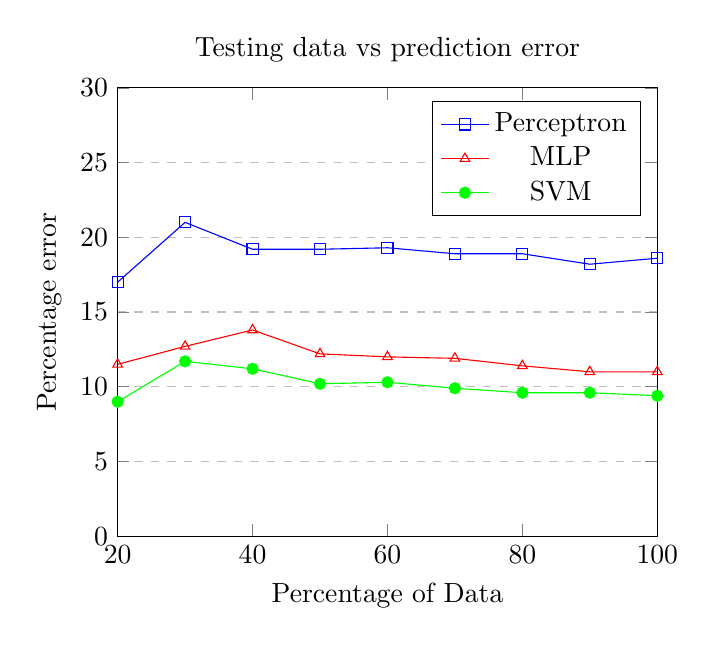
\begin{tikzpicture}
\begin{axis}[
    title={Testing data vs prediction error},
    xlabel={Percentage of Data},
    ylabel={Percentage error},
    xmin=20, xmax=100,
    ymin=0, ymax=30,
    xtick={20,40,60,80,100},
    ytick={0,5,10,15,20,25,30},
    legend pos=north east,
    ymajorgrids=true,
    grid style=dashed,
]
 
\addplot[
    color=blue,
    mark=square,
    ]
    coordinates {
    (20,17)(30,21)(40,19.2)(50,19.2)(60,19.3)(70,18.9)(80,18.9)(90,18.2)(100,18.6)
    };
    
\addplot[
    color=red,
    mark=triangle,
    ]
    coordinates {
    (20,11.5)(30,12.7)(40,13.8)(50,12.2)(60,12)(70,11.9)(80,11.4)(90,11)(100,11)
    };
    
\addplot[
    color=green,
    mark=*,
    ]
    coordinates {
    (20,9)(30,11.7)(40,11.2)(50,10.2)(60,10.3)(70,9.9)(80,9.6)(90,9.6)(100,9.4)
    };
    
    \legend{Perceptron,MLP, SVM}
 
\end{axis}
\end{tikzpicture}

\subsection*{5. Qualitative Evaluation}
One can see that the one layer perceptron does the worst. This makes sense since we know that a perceptron is equivalent to a non-linear line. Therefore, a single layer of perceptrons cannot make complex function. The SVM seems to do better than the MLP. SVM can often do better than MLP for lower dimensions such as this problem. Also using a premade library with default values may be tuned to these specific types of problems. I think if I play around a little more with the number of hidden nodes, and learning rate for MLP I can achieve better yields. For SVM using non default values may give me better results. Classical learning systems like neural networks suffer from their theoretical weakness, e.g. back-propagation usually converges only to locally optimal solutions. Here SVMs can provide a significant improvement.\\
For the training data size we see almost a linear decrease in error across all three learning methods. This shows that the more data we use to train the better our models become. Originally I had the learning rate as 0.5 for MLP and I was getting around 70-80\% test data results. After I changed it to 0.05 I started getting 85-90\%. Changing the number of hidden nodes and iterations did not have much effect on the error. As for SVM I thought the default values of gamma and C worked best.